\chapter{Grundlagen}
In diesem Kapitel werden das Vorgehensmodell und alle Tools, die für die erfolgreiche
Abwicklung des Projekts nötig sind, erläutert.

\section{Vorgehensmodelle}
Im Vorfeld der Durchführung des Projekts wurden Informationen über diverse Vorgehensmodelle
gesammelt. Für das Projektteam war schnell klar, dass ein agiles Modell gewählt werden sollte,
da somit das Projekt dynamischer geplant und durchgeführt werden kann. Die Auswahl für Scrum
stand direkt bei Projektbegin fest. In dem folgenden Abscnhitt wird dieses
Vorgehendsmodell genauer erklärt und unsere Entscheidung anschließend begründet.

\section{Scrum}
Scrum\footnote{Quelle: Scrum Alliance \cite{WHAT-IS-SCRUM}} repräsentiert ein agiles Projektmanagement-Framework,
das auf die effiziente Entwicklung von Produkten und Software abzielt. Es legt besonderen Wert auf Zusammenarbeit,
Anpassungsfähigkeit und die kontinuierliche Bereitstellung funktionsfähiger Inkremente innerhalb kurzer Entwicklungszyklen,
den sogenannten Sprints. \\

Die zuvor skizzierte Definition gewährt einen knappen Einblick in das agile Vorgehensmodell Scrum. Die herausragenden Merkmale dieses Modells sind:

\begin{itemize}
    \item Drei zentrale Rollen, die im Folgenden näher erläutert werden.
    \item Der Product Backlog, der sämtliche Anforderungen enthält.
    \item Eine iterative und zeitlich definierte Entwicklung von Produkten.
    \item Die autonome Arbeitsweise des Teams.
    \item Gleichberechtigung aller Teammitglieder.
\end{itemize}

\subsection{Die drei Rollen in Scrum}
\begin{itemize}
    \item \textbf{Product Owner}\footnote{Scrum-Rolle \cite{Product-Owner}}: Der Product Owner trägt die Verantwortung
    für die Pflege des Product Backlogs und vertritt dabei die fachliche Auftraggeberseite sowie sämtliche Stakeholder.
    Ein zentrales Anliegen ist die Priorisierung der Elemente im Product Backlog, um den geschäftlichen Wert des
    Produkts zu maximieren und die Möglichkeit für frühe Veröffentlichungen essenzieller Funktionalitäten zu schaffen.
    Der Product Owner nimmt nach Möglichkeit an den täglichen Scrum-Meetings teil, um auf passive Weise Einblicke zu
    gewinnen. Zudem steht er dem Team für Rückfragen zur Verfügung, um einen reibungslosen Informationsaustausch zu gewährleisten.
    \item \textbf{Scrum Master}\footnote{Scrum-Rolle \cite{Scrum-Master}}: Der Scrum Master übernimmt eine zentrale
    Rolle im Scrum-Prozess und ist für die korrekte Umsetzung desselben verantwortlich. Als Vermittler und Unterstützer
    fungiert er als Facilitator, der darauf abzielt, einen maximalen Nutzen zu erzielen und kontinuierliche Optimierung
    sicherzustellen. Ein zentrales Anliegen ist die Beseitigung von Hindernissen, um ein reibungsloses Voranschreiten
    des Teams zu gewährleisten. Der Scrum Master sorgt für einen effizienten Informationsfluss zwischen dem Product Owner
    und dem Team, moderiert Scrum-Meetings und behält die Aktualität der Scrum-Artefakte wie Product Backlog,
    Sprint Backlog und Burndown Charts im Blick. Darüber hinaus liegt in seiner Verantwortung, das Team vor
    unberechtigten Eingriffen während des Sprints zu schützen.
    \item \textbf{Team}\footnote{Scrum-Rolle \cite{Team}}: Das Team, bestehend aus vier bis zehn Mitgliedern,
    idealerweise sieben, zeichnet sich durch eine interdisziplinäre Zusammensetzung aus, die Entwickler, Architekten,
    Tester und technische Redakteure einschließt. Durch Selbstorganisation agiert das Team eigenständig und übernimmt
    die Verantwortung als sein eigener Manager. Es besitzt die Befugnis, autonom über die Aufteilung von Anforderungen
    in Aufgaben zu entscheiden und diese auf die einzelnen Mitglieder zu verteilen, wodurch der Sprint Backlog aus dem
    aktuellen Teil des Product Backlog entsteht.
\end{itemize}

\noindent Alle Anforderungen an das Produkt werden in sogenannten User Stories, vorrangig erstellt durch den Product
Owner, im Product Backlog gesammelt. In einem Intervall, bezeichnet als Sprint, werden die User Stories abgearbeitet.
Die Projektentwicklung nach Scrum besteht aus fünf zentralen Elementen:
\begin{itemize}
    \item \textbf{Sprint: Planning Meeting}\footnote{Scrum-Meetings \cite{Sprint-planing-meeting}}: Im Sprint Planning
    Meeting wird das Ziel des folgenden Sprints definiert. Hierbei werden die Anforderungen im Project Backlog, die in
    diesem Sprint umgesetzt werden sollen, in einzelne Aufgaben zerlegt und anschließend im Sprint Backlog gesammelt.
    \item \textbf{Sprint}\footnote{Scrum-Meetings \cite{Sprint}}: Ein Sprint repräsentiert eine Entwicklungsphase,
    während der eine voll funktionsfähige und potenziell veröffentlichte Software entsteht. Die Dauer eines solchen
    Sprints beträgt typischerweise zwischen 1 und 4 Wochen.
    \item \textbf{Daily Scrum}\footnote{Scrum-Meetings \cite{Daily-Scrum}}: Der Daily Scrum ist ein kurzes Teammeeting,
    in dem Teammitglieder darüber informieren, welche Aufgaben seit dem letzten Meeting abgeschlossen wurden, woran bis
    zum nächsten Meeting gearbeitet werden muss und wo momentane Probleme existieren. Auf diese Weise sind alle Teammitglieder
    stets auf dem aktuellen Stand, was die Lösung aufkommender Probleme erleichtert.
    \item \textbf{Sprint Review}\footnote{Scrum-Meetings \cite{Sprint-Review}}: In diesem Meeting präsentiert das
    Entwicklungsteam die im Sprint abgeschlossenen Arbeitsergebnisse, beispielsweise fertige Produktinkremente, den
    Stakeholdern, zu denen Produktbesitzer, Kunden, Führungskräfte und andere Interessengruppen gehören.
    \item \textbf{Sprint Retrospective}\footnote{Scrum-Meetings \cite{Sprint-Retroperspektiv}}: Die Sprint Retrospective
    dient primär dazu, dass das Scrum-Team (bestehend aus dem Entwicklungsteam, dem Scrum Master und dem Product Owner)
    gemeinsam den abgeschlossenen Sprint reflektiert und Möglichkeiten zur kontinuierlichen Verbesserung identifiziert.
\end{itemize}

\noindent Durch diese Elemente kann ein optimaler Projektablauf gewährleistet werden. Das Projekt bleibt jederzeit
offen für Änderungen, und durch eine enge Zusammenarbeit mit dem Kunden können Missverständnisse und Probleme
frühzeitig behandelt und kommuniziert werden.

\subsection{Begründung der Auswahl}
Die Applied Augmented Reality in Education Applikation besteht aus 3 verschiedenen Level.
Im Team welches aus vier Schülern bestand übernahm jede Person einen Teilbereich oder arbeiteten
gemeinsam an einem dieser Level mit Unteraufgaben in diesem Level. Unterstützt wurde man von einem
Lehrer, der stetz für Fragen bereitstand und oftmals in beratender Form vorhanden war. Als
Vorgehensmodell wählte das Team das agile Modell Scrum. Die von Scrum gegebenen Richtlinien
konnten leicht eingehalten werden, da das Team täglich in der Schule aufeinander
traf als auch privat Kontakt hatten. Jederart Änderung, Problem oder Änderungen und anderartige
Dinge konnten daher leicht kommuniziert und besprochen werden. Am Ende jedes Sprints wurden
die erreichten Ergebnisse mit dem Betreuer besprochen, sowie die Neuerungen vorgestellt.
In den Sprintreviews konnte somit Feedback zu den Ergebnissen gesammelt werden und von dem
Betreuer konnten neue Ansichten und Denkweisen angebracht und integriert werden.
Durch die Sprint Retroperspektive konnten die Schüler einen größeren Mehrwert aus der
Projektentwicklung schöpfen, da sie neben der Verwendung des Scrum-Prozesses auch ihre Fähigkeiten
in den einzelnen Bereichen, durch das Besprechen der positiven und negativen Aspekte verbessern.

\section{Projektmanagement-Tools}
Um einen positiven Verlauf des Projekts zu ermöglichen, benötigt man die unterstützenden
Tools beim Projektmanagement sowie die Verwaltung von Dateien.

\subsection{GitHub}
Als sogenanntes Repository für die Source Code Dateien wurde GitHub mit der dazugehörigen
Webanwendung verwendet. Zu Beginn des Projekts stand die Entscheidung an, welche Technologie
und welcher Anbieter für das Versionskontrollsystem gewählt werden sollten. Neben GitHub gibt es
andere namhafte Anbieter solcher Verwaltungssysteme, darunter GitLab und SourceForge.

Ausschlaggebend für die Wahl von GitHub waren mehrere Punkte. Zum einen ist GitHub eine
kostenlose Lösung, die es ermöglicht, ein privates Projekt mit mehreren Mitgliedern
ohne Kosten anzulegen. Im Gegensatz dazu bieten manche Plattformen nur eine begrenzte Anzahl
von Mitgliedschaften in kostenfreien Projekten an. Die Registrierung erforderte lediglich
einen Account.

Darüber hinaus bietet GitHub eine benutzerfreundliche Oberfläche, eine breite Unterstützung
für verschiedene Programmiersprachen und eine aktive Entwicklergemeinschaft. Dies erleichtert
die Zusammenarbeit und den Informationsaustausch im Projektteam.

\subsection{Jira}
Als sogenanntes Verwaltungstool für die Vorgänge im Projekt wurde Jira mit der dazugehörigen
Webanwendung verwendet. Auch hier stand zu Projektbeginn die Frage im Raum, welche Technologie
und welcher Anbieter für das Aufgabenmanagement gewählt werden sollten. Neben Jira gibt es
weitere namhafte Anbieter solcher Tools, darunter VivifyScrum und KanBan.

Die Wahl von Jira basierte auf mehreren Überlegungen. Zum einen ist Jira eine kostenlose
Lösung, die es ermöglicht, ein SCRUM Board mit mehreren Mitgliedern kostenfrei anzulegen.
Ein weiterer entscheidender Faktor war die direkte Verbindung zu dem GitHub-Repository und die Möglichkeit,
neue Branches und Commits direkt in Jira zu erstellen.

Darüber hinaus bietet Jira eine umfassende Funktionalität für das Projektmanagement, einschließlich
der Verfolgung von Aufgaben, der Planung von Sprints und der Erstellung von Berichten. Diese Features
ermöglichen es dem Projektteam, den Fortschritt genau zu überwachen und eventuelle Herausforderungen
frühzeitig zu identifizieren und anzugehen.

\section{Konzeption von Fragebögen}
Bei jeder Umfrage werden Informationen von Personen oder Personengruppen zu der allgemeinen
Umsetzung und dem Verständis der Applikation gesammelt. Diese werden im Anschluss ausgewertet und
interpretiert. Wichtig ist hier den Zweck jeder Umfrage genau zu definieren. Durch präzise und
detailierte Zielsetzungen ist es später dann möglich, den Erfolg der Umfrage zu garantieren.

\subsection{Planung der Fragebogenkonstruktion}

Die sorgfältige Konzeption und Gestaltung eines Fragebogens ist ein grundlegender Schritt bei der Planung einer Erhebung.
Eine genaue Planung stellt nicht nur sicher, dass relevante Daten erhoben werden. Sie erleichtert auch die spätere
Auswertung. Im Vorfeld werden daher verschiedene Entscheidungen getroffen und Definitionen festgelegt:

\begin{enumerate}

    \item \textbf{Inhalt:}
    Für die Qualität der erhobenen Daten ist die Auswahl der Inhalte von entscheidender Bedeutung. Es sollte die
    Möglichkeit in Betracht gezogen werden, bestehende Fragebögen zu verwenden. Gegebenenfalls sollten diese an die
    spezifischen Anforderungen der Erhebung angepasst werden. Die Fragen müssen klar und prägnant formuliert sein, um
    Missverständnisse zu vermeiden. Die Verwendung von validierten Fragebögen kann dazu beitragen, die Vergleichbarkeit
    mit anderen Studien zu gewährleisten.

    \item \textbf{Umfang:}
    Ein entscheidender Faktor, der in Abhängigkeit von den Forschungszielen abgewogen werden muss, ist die Länge des
    Fragebogens. Ziel sollte ein ausgewogenes Verhältnis zwischen der Tiefe der Informationen und der Aufrechterhaltung
    der Beteiligung der Teilnehmer sein. Ein zu umfangreicher Fragebogen kann die Ermüdung der Befragten und die
    Beeinträchtigung der Qualität der Antworten zur Folge haben.

    \item \textbf{Ablauf und zeitlicher Rahmen:}
    Die Entscheidung über den Ablauf und den zeitlichen Rahmen des Fragebogens beeinflusst die Art der Datenerhebung.
    Die Wahl zwischen einer postalischen Befragung und einer elektronischen Befragung wirkt sich auf die Zeit für die
    Beantwortung und die Effizienz der Datenerhebung aus. Elektronische Erhebungen liefern oft schnellere Ergebnisse,
    während postalische Erhebungen längere Rücklaufzeiten ermöglichen.

    \item \textbf{Zielgruppe:}
    Die Definition der Zielgruppe ist für die Repräsentativität der Ergebnisse von entscheidender Bedeutung. Ob eine
    Vollerhebung erfolgt oder eine Stichprobe gezogen wird, hängt von den verfügbaren Ressourcen und den spezifischen
    Forschungszielen ab. Eine Vollerhebung kann eine umfassende Datenbasis liefern, während eine Stichprobenerhebung
    effizienter sein kann, insbesondere wenn es sich um große Zielgruppen handelt.

    \item \textbf{Fragetypen und Antwortskalen:}
    Die Qualität der erhobenen Daten wird durch die Auswahl der Fragetypen und Antwortskalen beeinflusst. Geschlossene
    Fragen mit vorgegebenen Antwortmöglichkeiten erleichtern die quantitative Analyse, während offene Fragen die
    Möglichkeit bieten, qualitative Einsichten zu gewinnen. Die Wahl der Antwortskalen sollte auf die spezifischen
    Forschungsziele abgestimmt sein, unabhängig davon, ob es sich um Likert-Skalen oder numerische Bewertungen handelt.

    \item \textbf{Ethik und Datenschutz:}
    Ethische Aspekte, wie die Anonymität der Teilnehmer zu wahren und sensible Informationen zu schützen, sind von
    entscheidender Bedeutung. Das Design des Fragebogens sollte so sein, dass die Integrität der Teilnehmer gewahrt wird
    und keine unangemessenen persönlichen Informationen gesammelt werden.

    \item \textbf{Pilotstudie:}
    Es wird empfohlen, vor der endgültigen Implementierung des Erhebungsbogens eine Pilotstudie durchzuführen. In dieser
    Testphase können mögliche Probleme, Unklarheiten oder Missverständnisse in den Fragen identifiziert und behoben werden.
    Das Feedback der Testteilnehmer trägt zur Optimierung des Fragebogens bei.
\end{enumerate}
\\

Um das Verständnis der Planung der Fragebögen als auch der Formulierungen der einzelnen Fragen zu erleichtern, enthält
dieser Abschnitt ein \textit{Fallbeispiel}, welches für nähere Erklärungen herangezogen wird:
\begin{quote}
    Während des Tages der offenen Tür (an dem 25 Personen die Anwendung testeten) und in einer Abschlussklasse einer
    maturaführenden Schule wird eine Umfrage durchgeführt. Ziel der Umfrage ist es, die Meinung der Benutzer über die
    aktuelle Anwendung zu erfahren. Es soll festgestellt werden, ob die Grundidee verstanden wurde und ob es etwas zu
    verbessern gäbe. Eine quantitative Untersuchung zeigt, dass ein Drittel der Personen, die am Tag der offenen Tür
    teilgenommen haben, das vermittelte Konzept verstanden haben und keine Vorschläge für Verbesserungen haben. Die
    Personen der Abschlussklasse zeigen, dass sie das Vermittelte verstanden haben und haben auch Verbesserungsvorschläge.
    Anschließend wurden 5 Schülerinnen und Schüler der Klasse befragt (Stichprobe). Ziel war es, die Gründe für einige
    Verbesserungsvorschläge herauszufinden. Das Ergebnis zeigt, dass alle Befragten viele Verbesserungsvorschläge haben.
    Der Grund dafür ist, dass aufgrund des frühen Entwicklungsstadiums viele Dinge noch nicht zu Ende entwickelt wurden
    oder noch nicht in der Umsetzung sind.
\end{quote}
\\

Grundsätzlich werden die \textit{quantitative} und die \textit{qualitative Forschung} unterschieden, wobei Fragebögen
zur \textit{quantitativen Forschung} aufgrund der besseren Vergleichbarkeit leichter zu interpretieren sind.

Bei der Quantifizierung schließt man von der Stichprobe auf die Grundgesamtheit N, wie in Abbildung 2.2 gezeigt. Es ist
wichtig, dass die ausgewählte Stichprobe repräsentativ ist. Das bedeutet, dass die Personen, die an der Stichprobe
teilnehmen, die gleichen Voraussetzungen haben wie die Personen, die tatsächlich in der Grundgesamtheit vorkommen. Es
handelt sich hierbei um numerische Daten, die erhoben werden und für die eine Auswertung vorgenommen wird. Von Bedeutung
ist in diesem Zusammenhang das Verhältnis zwischen der untersuchten Stichprobe und der Grundgesamtheit (Population). In
diesem Zusammenhang ist das Verhältnis zwischen der untersuchten Auswahl und der Population von Bedeutung. Alle Merkmale
der Personen in der Auswahl müssen mit den Merkmalen der Personen in der Population übereinstimmen, zum Beispiel Alter
und Geschlecht.\footnote{Vgl. Mayer, \cite{Interview und schriftliche Befragung}, S. 57 ff.}

%Hier Bild für den Zusammenhand
\begin{figure}[h]
    \centering
    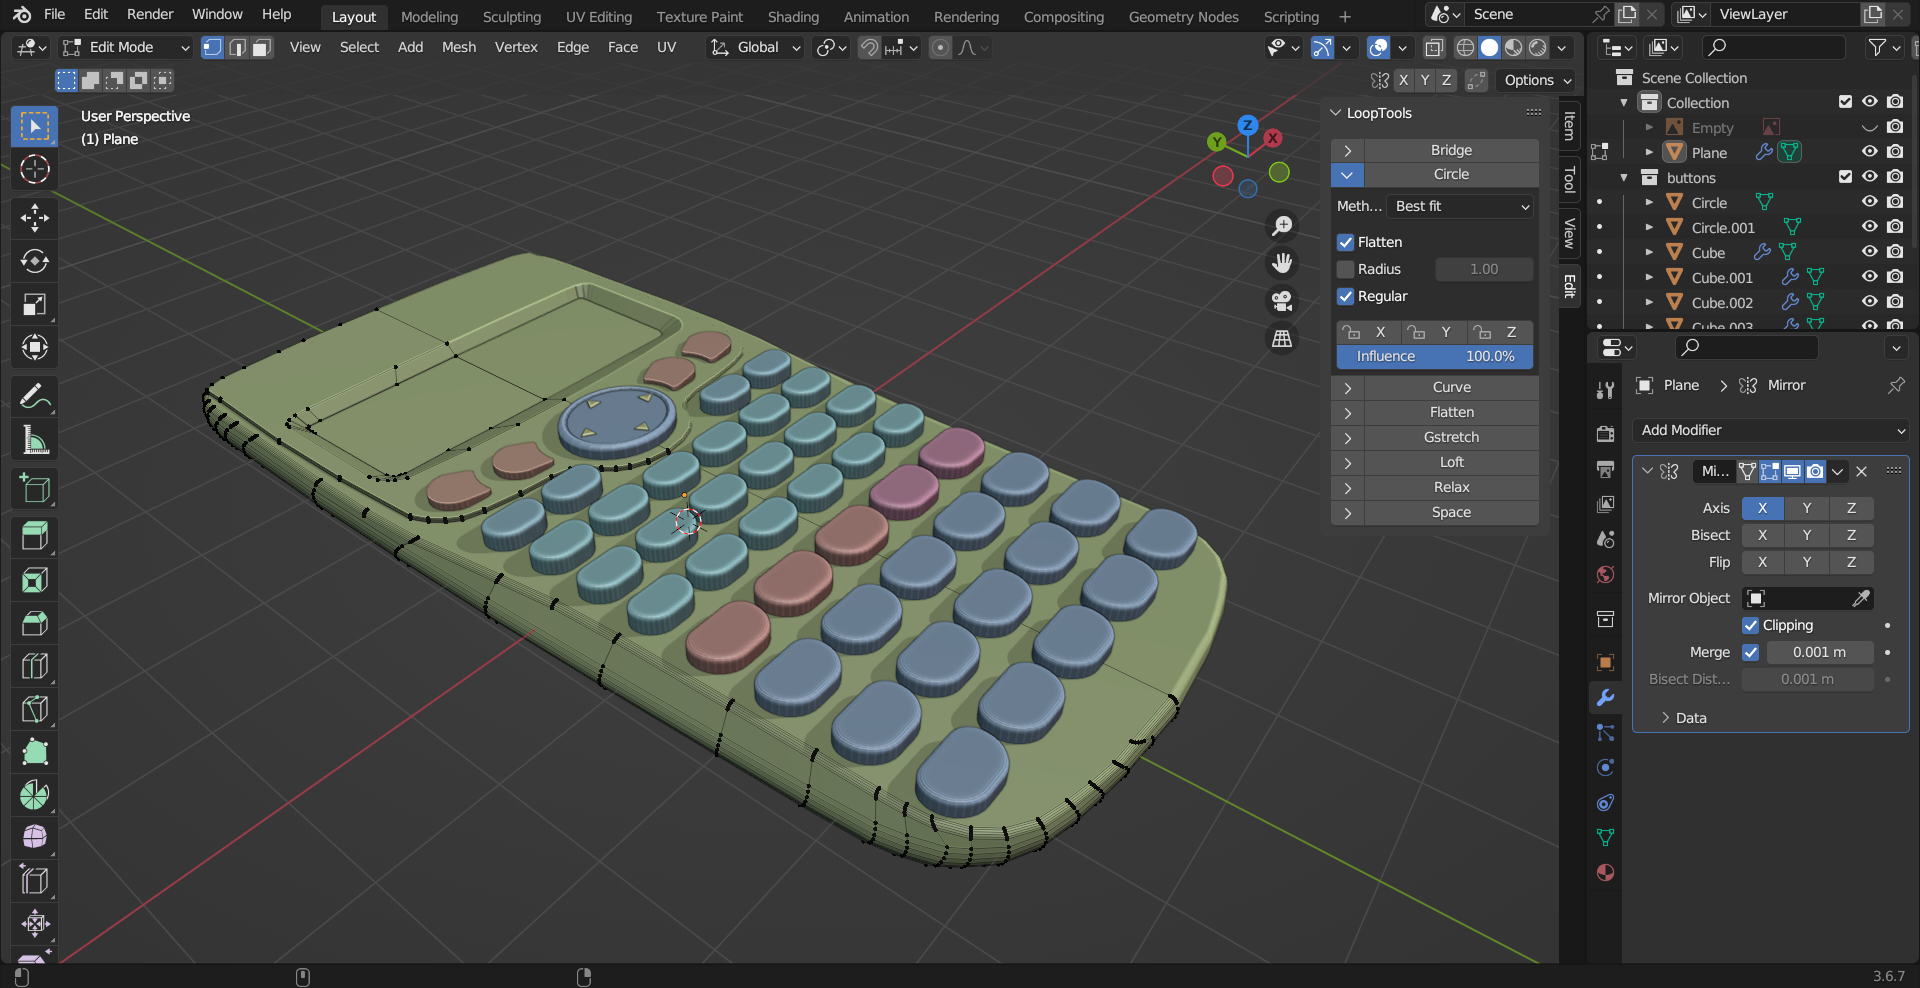
\includegraphics[width=1\textwidth]{images/calculatoreditmode.png}
    \caption{Zusammenhang zwischen der \textit{Grundgesameheit} und \textit{Stichprobe}}
    \label{fig:calculatoreditmode}
\end{figure}

Anhand des Fallbeispiels wird verdeutlicht, dass es keinen Sinn macht, die Umfrage an sehr jungen Leuten durchzuführen,
da diese Personen zum größten Teil noch nicht wirklich tiefer in die Informatik geblickt haben und dadurch diese Prinzipien
nicht verständlich sind.

Die qualitative Forschung ist eine Methode zur Auswertung von Daten, die ausschließlich über Sprache (verbal) übermittelt
werden. Diese Methode eignet sich vor allem zur näheren Beschreibung und Analyse von subjektiven Wahrnehmungen,
persönlichen Einstellungen, Motiven und Meinungen der Befragten.\footnote{Vgl. Mayer, \cite{Interview und schriftliche Befragung}, S. 36}

Am sinnvollsten ist eine Kombination von \textit{qualitativen und quantitativen Ergebnissen}. Nach einer quantitativen
Befragung sollte eine stichprobenartige qualitative Befragung durchgeführt werden, um die Ergebnisse besser
interpretieren zu können. Dies wird anhand eines Fallbeispiels veranschaulicht.

Unabhängig davon, ob es sich um qualitative oder quantitative Forschung handelt, sind die drei \textit{Gütekriterien
Objektivität, Zuverlässigkeit und Validität} zu erfüllen.

Sie dienen, den Forschungsprozess zu steuern und zu kontrollieren. Die Validität ist ein Maß für die Brauchbarkeit der
Methode und bezieht sich auf die tatsächliche Fähigkeit zur Messung des gewünschten Wertes. Das Ergebnis ist umso
zuverlässiger, je klarer die Fragen formuliert sind. Entscheidend für die Validität der Analyse ist die Objektivität
der Messung. Dabei ist sowohl die Durchführungsobjektivität des Befragers als auch die Auswertungs- und
Interpretationsobjektivität des Analytikers zu beachten.\footnote{Vgl. Mayer, \cite{Interview und schriftliche Befragung}, S. 54 ff., S. 88.}

Die drei Gütekriterien stehen in einem wechselseitigen Zusammenhang. Nur, wenn die Objektivität gegeben ist, kann die
Reliabilität gewährleistet werden. Ist die Reliabilität gering, kann die Validität nur mit einer gewissen Unsicherheit
vorhergesagt werden.\footnote{Vgl. Bühner, \cite{Einfuehrung in die Test- und Fragebogenkonstruktion}, S. 33 f.}

\subsection{Formulierung der Fragen}
Um eine erfolgreiche Umfrage effizient durchführen zu können, ist eine sorgfältige Vorbereitung erforderlich. Die
Erkenntnis, dass Umfragen nur bestimmte Aspekte eines Themenbereichs abdecken können, ist von entscheidender Bedeutung.
Aus diesem Grund ist eine sorgfältige und präzise Definition dieser Aspekte erforderlich. Besonderes Augenmerk ist darauf
zu richten, dass die Fragen klar formuliert sind.

Die zentrale Priorität bei der Formulierung der Fragen ist die Verständlichkeit und Eindeutigkeit. Die folgenden
Formulierungsrichtlinien sollten unbedingt beachtet werden:
\begin{itemize}
    \item Verwendung von einfachem Vokabular ohne Verwendung von Fachausdrücken, Fremdwörtern oder Ausdrücken aus anderen Sprachen.
    \item Die Fragen prägnant formulieren.
    \item Belastende Begriffe wie "Ehrlichkeit" werden vermieden.
    \item Hypothetische Formulierungen sollten ausgeschlossen werden.
    \item Fokussierung auf ein bestimmtes Thema für jede einzelne Frage.
    \item Vermeidung von Überforderung durch die Bereitstellung einer angemessenen Menge an Informationen pro Frage.
    \item Doppelte Verneinungen sind zu vermeiden. \footnote{Vgl. Mayer, \cite{Interview und schriftliche Befragung}, S. 89.}\\
\end{itemize}

Die genannten Kriterien sind besonders wichtig bei schriftlichen Befragungen. Um sicherzustellen, dass die Ergebnisse
nicht verfälscht werden, darf der Interviewer keine zusätzlichen Fragen stellen oder die bereits gestellten Fragen ändern.

Direkte Fragen sind geeignet, um Fakten und Wünsche zu ermitteln, während formulierte Aussagen oder Feststellungen eher
dazu dienen, die Bewertung durch die Befragten in Erfahrung zu bringen. Diese Techniken werden hauptsächlich zur
Erfassung von Einstellungen, Wahrnehmungen und Meinungen eingesetzt.

\subsection{Arten von Fragen}
Je nach den Anforderungen der jeweiligen Auswertung wird zwischen offenen und geschlossenen Fragen unterschieden.

Bei offenen Fragen handelt es sich um Fragen, bei denen Antwortmöglichkeiten nicht vorgegeben sind. Im Anschluss an die
Frage sollte ausreichend Platz für die Beantwortung zur Verfügung stehen. Diese Art von Fragen sollte in den folgenden
Fällen verwendet werden:
\begin{itemize}
    \item Wenn die Zahl der Antwortmöglichkeiten nicht bekannt ist.
    \item Wenn die Formulierung der Antwort des Auskunftspflichtigen für die Auswertung wichtig ist.
    \item Wenn das Ziel der Erhebung darin besteht, die Unwissenheit und das Fehlen einer Meinung zu ermitteln.\\
\end{itemize}

Im Gegensatz zu offenen Fragen gibt es bei geschlossenen Fragen vordefinierte Antwortmöglichkeiten. Die Teilnehmenden
wählen ihre Antworten aus einer festgelegten Liste oder entscheiden sich zwischen vorgegebenen Optionen. Der Einsatz
geschlossener Fragen ist in verschiedenen Szenarien angebracht:

\begin{itemize}
    \item Wenn die Anzahl der möglichen Antwortalternativen bekannt und begrenzt ist.
    \item Bei Umfragen, bei denen quantitative Daten für eine statistische Auswertung erforderlich sind.
    \item Wenn die Standardisierung der Antworten wichtig ist, um eine konsistente Analyse zu ermöglichen.\footnote{Vgl. Scholl, \cite{Die Befragung}, S. 157.}\\
\end{itemize}

In Bezug auf die geschlossenen Fragen ist es noch wichtig anzumerken, dass es im Wesentlichen drei Möglichkeiten für die
Benennung oder Kennzeichnung gibt.
\begin{enumerate}
    \item \textbf{Numerische Benennung}
    Die numerische Benennung ist die Verwendung eines klassischen Notationssystems mit semantischer Bedeutung: Jede Note
    oder Zahl ist eindeutig einer sprachlichen Formulierung zugeordnet, wobei der Abstand zwischen den einzelnen Noten gleich groß ist.
    \item \textbf{Kennzeichnung durch Formen}
    Eine Möglichkeit, geschlossene Fragen zu kennzeichnen, besteht darin, bestimmte Formen wie Kreise, Kästchen oder
    grafische Skalen (Symbole) zu verwenden.
    \item \textbf{Sprachliche Benennung}
    Die sprachliche Benennung als Methode zur Kennzeichnung geschlossener Fragen bezieht sich auf die Verwendung von
    klaren sprachlichen Ausdrücken oder Texten, um die verschiedenen Antwortoptionen zu definieren. \footnote{Vgl. Mayer, \cite{Interview und schriftliche Befragung}, S. 164 ff.}
\end{enumerate}

%Offene und geschlossene Fragen erklären

\subsection{Struktur und Gliederung von Fragebögen}
Hier wird verfasst wie die Allgemeine Struktur und Gliederung von Fragebögen aussehen soll. \footnote{Vgl. \cite{Buehner} S. -}

\subsection{Mögliche Verfälschung des Resultats}
Welche Arten von Verfälschungen gibt es und diese Beschreiben
Ursachen dafür beschreiben. \footnote{Vgl. \cite{Buehner} S. -}

\subsection{Auswertung von Fragebögen}
Wie werten wir die Fragenbögen aus? \footnote{Vgl. \cite{Mayer} S. -}

%Quellen zu den Fragenbögen Dingen finden und ALLES genauer beschreiben
